
\documentclass[letterpaper,hide notes,xcolor={table,svgnames},pdftex,10pt]{beamer}
\def\showexamples{t}


%\usepackage[svgnames]{xcolor}

%% Demo talk
%\documentclass[letterpaper,notes=show]{beamer}

\usecolortheme{crane}
\setbeamertemplate{navigation symbols}{}

\usetheme{MyPittsburgh}
%\usetheme{Frankfurt}

%\usepackage{tipa}

\usepackage{hyperref}
\usepackage{graphicx,xspace}
\usepackage[normalem]{ulem}
\usepackage{multicol}
\usepackage{amsmath,amssymb,amsthm,graphicx,xspace}
\usepackage{ifsym}
\newcommand\SF[1]{$\bigstar$\footnote{SF: #1}}

\usepackage[default]{sourcesanspro}
\usepackage[T1]{fontenc}


\newcounter{tmpnumSlide}
\newcounter{tmpnumNote}

% old question code
%\newcommand\question[1]{{$\bigstar$ \small \onlySlide{2}{#1}}}
% \newcommand\nquestion[1]{\ifdefined \presentationonly \textcircled{?} \fi \note{\par{\Large \textbf{?}} #1}}
% \newcommand\nanswer[1]{\note{\par{\Large \textbf{A}} #1}}


 \newcommand\mnote[1]{%
   \addtocounter{tmpnumSlide}{1}
   \ifdefined\showcues {~\tiny\fbox{\arabic{tmpnumSlide}}}\fi
   \note{\setlength{\parskip}{1ex}\addtocounter{tmpnumNote}{1}\textbf{\Large \arabic{tmpnumNote}:} {#1\par}}}

\newcommand\mmnote[1]{\note{\setlength{\parskip}{1ex}#1\par}}

%\newcommand\mnote[2][]{\ifdefined\handoutwithnotes {~\tiny\fbox{#1}}\fi
% \note{\setlength{\parskip}{1ex}\textbf{\Large #1:} #2\par}}

%\newcommand\mnote[2][]{{\tiny\fbox{#1}} \note{\setlength{\parskip}{1ex}\textbf{\Large #1:} #2\par}}

\newcommand\mquestion[2]{{~\color{red}\fbox{?}}\note{\setlength{\parskip}{1ex}\par{\Large \textbf{?}} #1} \note{\setlength{\parskip}{1ex}\par{\Large \textbf{A}} #2\par}\ifdefined \presentationonly \pause \fi}

\newcommand\blackboard[1]{%
\ifdefined   \showblackboard
  {#1}
  \else {\begin{center} \fbox{\colorbox{blue!30}{%
         \begin{minipage}{.95\linewidth}%
           \hspace{\stretch{1}} Some space intentionally left blank; done at the blackboard.%
         \end{minipage}}}\end{center}}%
         \fi%
}



%\newcommand\q{\tikz \node[thick,color=black,shape=circle]{?};}
%\newcommand\q{\ifdefined \presentationonly \textcircled{?} \fi}

\usepackage{listings}
\lstset{%
  keywordstyle=\bfseries,
  aboveskip=15pt,
  belowskip=15pt,
  captionpos=b,
  identifierstyle=\ttfamily,
  escapeinside={(*@}{@*)},
  stringstyle=\ttfamiliy,
  frame=lines,
  numbers=left, basicstyle=\scriptsize, numberstyle=\tiny, stepnumber=0, numbersep=2pt}

\usepackage{siunitx}
\newcommand\sius[1]{\num[group-separator = {,}]{#1}\si{\micro\second}}
\newcommand\sims[1]{\num[group-separator = {,}]{#1}\si{\milli\second}}
\newcommand\sins[1]{\num[group-separator = {,}]{#1}\si{\nano\second}}
\sisetup{group-separator = {,}, group-digits = true}

%% -------------------- tikz --------------------
\usepackage{tikz}
\usetikzlibrary{positioning}
\usetikzlibrary{arrows,backgrounds,automata,decorations.shapes,decorations.pathmorphing,decorations.markings,decorations.text}

\tikzstyle{place}=[circle,draw=blue!50,fill=blue!20,thick, inner sep=0pt,minimum size=6mm]
\tikzstyle{transition}=[rectangle,draw=black!50,fill=black!20,thick, inner sep=0pt,minimum size=4mm]

\tikzstyle{block}=[rectangle,draw=black, thick, inner sep=5pt]
\tikzstyle{bullet}=[circle,draw=black, fill=black, thin, inner sep=2pt]

\tikzstyle{pre}=[<-,shorten <=1pt,>=stealth',semithick]
\tikzstyle{post}=[->,shorten >=1pt,>=stealth',semithick]
\tikzstyle{bi}=[<->,shorten >=1pt,shorten <=1pt, >=stealth',semithick]

\tikzstyle{mut}=[-,>=stealth',semithick]

\tikzstyle{treereset}=[dashed,->, shorten >=1pt,>=stealth',thin]

\usepackage{ifmtarg}
\usepackage{xifthen}
\makeatletter
% new counter to now which frame it is within the sequence
\newcounter{multiframecounter}
% initialize buffer for previously used frame title
\gdef\lastframetitle{\textit{undefined}}
% new environment for a multi-frame
\newenvironment{multiframe}[1][]{%
\ifthenelse{\isempty{#1}}{%
% if no frame title was set via optional parameter,
% only increase sequence counter by 1
\addtocounter{multiframecounter}{1}%
}{%
% new frame title has been provided, thus
% reset sequence counter to 1 and buffer frame title for later use
\setcounter{multiframecounter}{1}%
\gdef\lastframetitle{#1}%
}%
% start conventional frame environment and
% automatically set frame title followed by sequence counter
\begin{frame}%
\frametitle{\lastframetitle~{\normalfont(\arabic{multiframecounter})}}%
}{%
\end{frame}%
}
\makeatother

\makeatletter
\newdimen\tu@tmpa%
\newdimen\ydiffl%
\newdimen\xdiffl%
\newcommand\ydiff[2]{%
    \coordinate (tmpnamea) at (#1);%
    \coordinate (tmpnameb) at (#2);%
    \pgfextracty{\tu@tmpa}{\pgfpointanchor{tmpnamea}{center}}%
    \pgfextracty{\ydiffl}{\pgfpointanchor{tmpnameb}{center}}%
    \advance\ydiffl by -\tu@tmpa%
}
\newcommand\xdiff[2]{%
    \coordinate (tmpnamea) at (#1);%
    \coordinate (tmpnameb) at (#2);%
    \pgfextractx{\tu@tmpa}{\pgfpointanchor{tmpnamea}{center}}%
    \pgfextractx{\xdiffl}{\pgfpointanchor{tmpnameb}{center}}%
    \advance\xdiffl by -\tu@tmpa%
}
\makeatother
\newcommand{\copyrightbox}[3][r]{%
\begin{tikzpicture}%
\node[inner sep=0pt,minimum size=2em](ciimage){#2};
\usefont{OT1}{phv}{n}{n}\fontsize{4}{4}\selectfont
\ydiff{ciimage.south}{ciimage.north}
\xdiff{ciimage.west}{ciimage.east}
\ifthenelse{\equal{#1}{r}}{%
\node[inner sep=0pt,right=1ex of ciimage.south east,anchor=north west,rotate=90]%
{\raggedleft\color{black!50}\parbox{\the\ydiffl}{\raggedright{}#3}};%
}{%
\ifthenelse{\equal{#1}{l}}{%
\node[inner sep=0pt,right=1ex of ciimage.south west,anchor=south west,rotate=90]%
{\raggedleft\color{black!50}\parbox{\the\ydiffl}{\raggedright{}#3}};%
}{%
\node[inner sep=0pt,below=1ex of ciimage.south west,anchor=north west]%
{\raggedleft\color{black!50}\parbox{\the\xdiffl}{\raggedright{}#3}};%
}
}
\end{tikzpicture}
}


%% --------------------

%\usepackage[excludeor]{everyhook}
%\PushPreHook{par}{\setbox0=\lastbox\llap{MUH}}\box0}

%\vspace*{\stretch{1}

%\setbox0=\lastbox \llap{\textbullet\enskip}\box0}

\setlength{\parskip}{\fill}

\newcommand\noskips{\setlength{\parskip}{1ex}}
\newcommand\doskips{\setlength{\parskip}{\fill}}

\newcommand\xx{\par\vspace*{\stretch{1}}\par}
\newcommand\xxs{\par\vspace*{2ex}\par}
\newcommand\tuple[1]{\langle #1 \rangle}
\newcommand\code[1]{{\sf \footnotesize #1}}
\newcommand\ex[1]{\uline{Example:} \ifdefined \presentationonly \pause \fi
  \ifdefined\showexamples#1\xspace\else{\uline{\hspace*{2cm}}}\fi}

\newcommand\ceil[1]{\lceil #1 \rceil}


\AtBeginSection[]
{
   \begin{frame}
       \frametitle{Outline}
       \tableofcontents[currentsection]
   \end{frame}
}



\pgfdeclarelayer{edgelayer}
\pgfdeclarelayer{nodelayer}
\pgfsetlayers{edgelayer,nodelayer,main}

\tikzstyle{none}=[inner sep=0pt]
\tikzstyle{rn}=[circle,fill=Red,draw=Black,line width=0.8 pt]
\tikzstyle{gn}=[circle,fill=Lime,draw=Black,line width=0.8 pt]
\tikzstyle{yn}=[circle,fill=Yellow,draw=Black,line width=0.8 pt]
\tikzstyle{empty}=[circle,fill=White,draw=Black]
\tikzstyle{bw} = [rectangle, draw, fill=blue!20,
    text width=4em, text centered, rounded corners, minimum height=2em]

    \newcommand{\CcNote}[1]{% longname
	This work is licensed under the \textit{Creative Commons #1 3.0 License}.%
}
\newcommand{\CcImageBy}[1]{%
	\includegraphics[scale=#1]{creative_commons/cc_by_30.pdf}%
}
\newcommand{\CcImageSa}[1]{%
	\includegraphics[scale=#1]{creative_commons/cc_sa_30.pdf}%
}
\newcommand{\CcImageNc}[1]{%
	\includegraphics[scale=#1]{creative_commons/cc_nc_30.pdf}%
}
\newcommand{\CcGroupBySa}[2]{% zoom, gap
	\CcImageBy{#1}\hspace*{#2}\CcImageNc{#1}\hspace*{#2}\CcImageSa{#1}%
}
\newcommand{\CcLongnameByNcSa}{Attribution-NonCommercial-ShareAlike}

\newenvironment{changemargin}[1]{%
  \begin{list}{}{%
    \setlength{\topsep}{0pt}%
    \setlength{\leftmargin}{#1}%
    \setlength{\rightmargin}{1em}
    \setlength{\listparindent}{\parindent}%
    \setlength{\itemindent}{\parindent}%
    \setlength{\parsep}{\parskip}%
  }%
  \item[]}{\end{list}}




\title{Tutorial 1}

\author{Richard Wong \\ \small \texttt{rk2wong@edu.uwaterloo.ca}}
\institute{Department of Electrical and Computer Engineering \\
  University of Waterloo}
\date{\today}


\begin{document}

\begin{frame}
  \titlepage

\end{frame}


\begin{frame}
\frametitle{How to Best Make Use of Tutorials}

Treat material presented in these slides as a supplement to Prof. Zarnett's lecture slides, given from a slightly different perspective.

If you notice that this perspective could be wrong, don't hesitate to speak up!

We will also walk through some exercises in tutorial to serve as practice.

\end{frame}

\begin{frame}
\frametitle{The Entity-Relationship Model}

In short, this model lets us represent:\\
\begin{itemize}
  \item tables in a database with \textbf{mathematical sets}, and
  \item queries on the database with a language called the \textbf{relational algebra}.
\end{itemize}

\end{frame}


\begin{frame}
\frametitle{Nouns of the Relational Model (1/2)}

A \textbf{relation} $R$ is equivalent to a table.

An \textbf{attribute} $A$ is equivalent to a column of a table.

We describe the combination of relation and attributes with a \textbf{relation schema} of the form $R(A_1, A_2, ... , A_n)$.

$Student(student\_number, name, address)$ tells us:\\
\begin{itemize}
  \item there is a table called \texttt{Student}, and
  \item it has attributes \texttt{name} and \texttt{address}.
\end{itemize}

\texttt{name} is an attribute of the relation \texttt{Student}.

\end{frame}

\begin{frame}
\frametitle{Nouns of the Relational Model (2/2)}

The \textbf{contents} of a relation $R$ are denoted $r(R)$.

$r(R)$ is an (unordered) set of (ordered) \textbf{n-tuples}.

Each \textbf{n-tuple} of $r(R)$ is equivalent to a row in the relation/table $R$.

The elements of each n-tuple correspond with the attributes $A_1, A_2, ... , A_n$ of $R$.

\end{frame}

\begin{frame}
\frametitle{Nouns of the Entity-Relationship Model (1/5)}

An \textbf{entity} [table] is equivalent to a relation, which is equivalent to a table.\\
\begin{itemize}
  \item \texttt{Student} can be an entity in an E-R model.
\end{itemize}

However, we also use the term \textbf{entity} to describe an object in the real world, indistinguishable from other objects.\\
\begin{itemize}
  \item A student with student number 20000000 and name Matt is an entity of type \texttt{Student}.
\end{itemize}

In this way, an entity [object] is equivalent to a row of an entity [table].

\end{frame}


\begin{frame}
\frametitle{Nouns of the Entity-Relationship Model (2/5)}

An \textbf{entity set} is a set of entities (in the object sense), and is equivalent to the contents of an entity table.\\
\begin{itemize}
  \item The set of all students studying at the University of Waterloo might comprise the entity set \texttt{Student}.
\end{itemize}

For instance, \texttt{Student} = \{(20000000, Matt), (20000001, Josh)\}

\end{frame}


\begin{frame}
\frametitle{Nouns of the Entity-Relationship Model (3/5)}

Suppose we have another entity called \texttt{Course}, with attributes \texttt{course\_id} and \texttt{title}.

Then the following are two possible entity sets:\\
\texttt{Student} = \{(20000000, Matt), (20000001, Josh)\}\\
\texttt{Course} = \{(CS101, Intro to CS), (CS999, Super Hard CS)\}

A \textbf{relationship} describes some connection between entities, in both the table sense and the object sense.\\
\begin{itemize}
  \item In our E-R model, we can say \texttt{Student} takes \texttt{Course}.
  \item An individual student like Matt can take a course like Intro to CS.
\end{itemize}
\end{frame}


\begin{frame}
\frametitle{Nouns of the Entity-Relationship Model (4/5)}

A \textbf{relationship instance} describes how two entity instances are related. The following are each relationship instances:
\begin{itemize}
  \item Matt takes Intro to CS: $takes_1$ = ((20000000, Matt), (CS101, Intro to CS))
  \item Josh also takes Intro to CS: $takes_2$ = ((20000001, Josh), (CS101, Intro to CS))
  \item Intro to CS is taught by Prof. X: $taughtby_1$ = ((CS101, Intro to CS), (1, Prof. X))
\end{itemize}


A \textbf{relationship set} is a set of relationship instances.\\
\begin{itemize}
  \item In an E-R model, a relationship set represents how entities (in the table sense) are related.
  \begin{itemize}
    \item \texttt{Student}s take \texttt{Courses}: $Takes$ = \{$takes_1, takes_2$\}
    \item \texttt{Courses} are taught by \texttt{Instructors}: $TaughtBy$ = \{$taughtby_1$\}
  \end{itemize}
\end{itemize}

In an E-R model, we can use a table to represent a relationship set.\\
Such a table will have columns to identify which entities are related.\\
\begin{itemize}
  \item The \texttt{StudentTakesCourse} table might have columns for \texttt{student\_id} and \texttt{course\_id}.
  \item This represents a relationship of \textbf{degree} 2, since it relates 2 entities.
\end{itemize}

\end{frame}


\begin{frame}
\frametitle{Nouns of the Entity-Relationship Model (5/5)}

An \textbf{attribute} is data used to describe an entity.

Attributes have a set of legal values called a \textbf{domain}, determined by the data type we ascribe to them in our relational schema.

\textbf{Simple attributes} contain a single value, e.g. \texttt{INT}, \texttt{VARCHAR(20)}, \texttt{ENUM}.

\textbf{Composite attributes} encapsulate other simple or composite attributes. Think someething similar to C \texttt{struct}s.
\begin{itemize}
  \item A composite attribute like an \texttt{Address} can be composed of the following attributes:
  \begin{itemize}
    \item lot number,
    \item street,
    \item nullable apartment/unit number,
    \item city,
    \item province/state,
    \item country, and
    \item postal code.
  \end{itemize}
\end{itemize}

\end{frame}


\begin{frame}
\frametitle{A Note About \texttt{NULL}}

Use <column> \texttt{IS NULL} or <column> \texttt{IS NOT NULL} to perform null checks.

It typically does not make sense to have any other operators on \texttt{NULL} values.

Treat \texttt{NULL} as "not having a value", as opposed to an "empty value" like 0 or "".

\end{frame}


\begin{frame}
\frametitle{Let's get some exercise! - E-R Modeling}

Translate the following E-R diagram into a set of database tables by writing relational schemas:

\begin{center}
  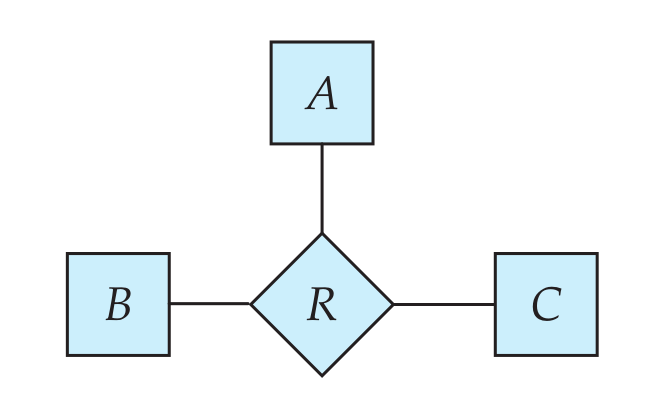
\includegraphics[width=0.7\textwidth]{images/ternary-relationship.png}
\end{center}

\end{frame}


\begin{frame}
\frametitle{Let's get some exercise! - E-R Modeling}

Translate the following E-R diagram into a set of database tables by writing relational schemas:

\begin{center}
  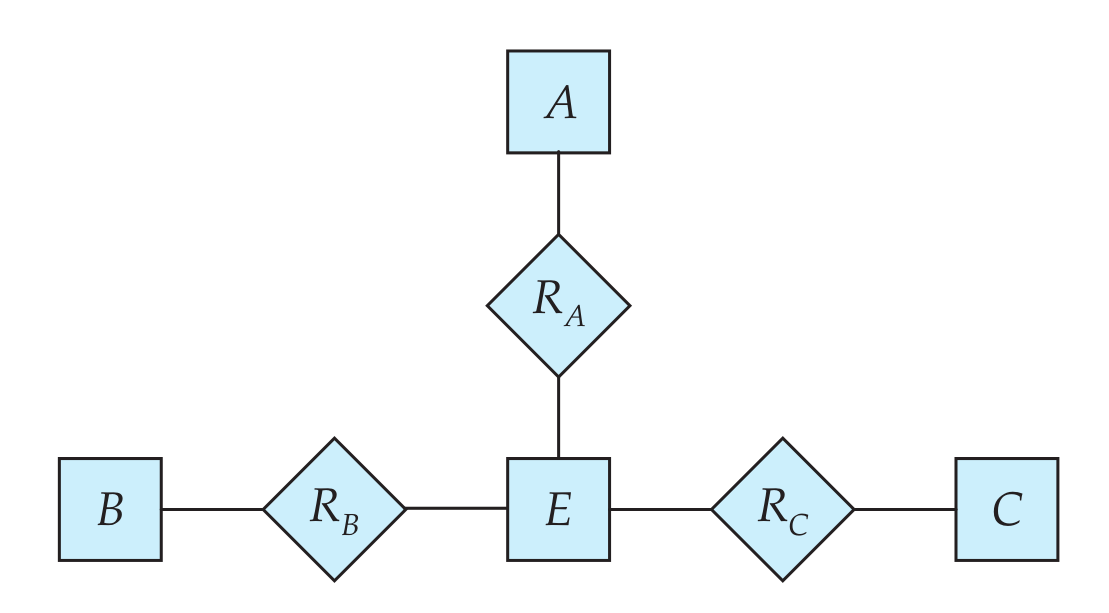
\includegraphics[width=0.7\textwidth]{images/three-binary-relationships.png}
\end{center}

\end{frame}


\begin{frame}
\frametitle{Let's get some exercise! - E-R Modeling}

Draw an E-R diagram to represent the following database specification for a simple Quest-like system:\\
\begin{itemize}
  \item Students are identified by student numbers, and have names.
  \item Courses have course codes and titles.
  \item Courses are offered in a given term (W, S, F) in a given year.
  \item Courses are offered in one or more sections.
  \item Students enroll in sections of a course.
  \item Students get grades for the sections they are enrolled in at the end of a term.
\end{itemize}

\end{frame}


\begin{frame}
\frametitle{Let's get some exercise! - E-R Modeling}

Sketch out the tables that would implement your E-R diagram for the following specification:\\
\begin{itemize}
  \item Students are identified by student numbers, and have names.
  \item Courses have course codes and titles.
  \item Courses are offered in a given term (W, S, F) in a given year.
  \item Courses are offered in one or more sections.
  \item Students enroll in sections of a course.
  \item Students get grades for the sections they are enrolled in at the end of a term.
\end{itemize}

\end{frame}


\begin{frame}
\frametitle{Let's get some exercise! - Relational Queries}

Let's say we're given the following schema for a university database:

\begin{center}
  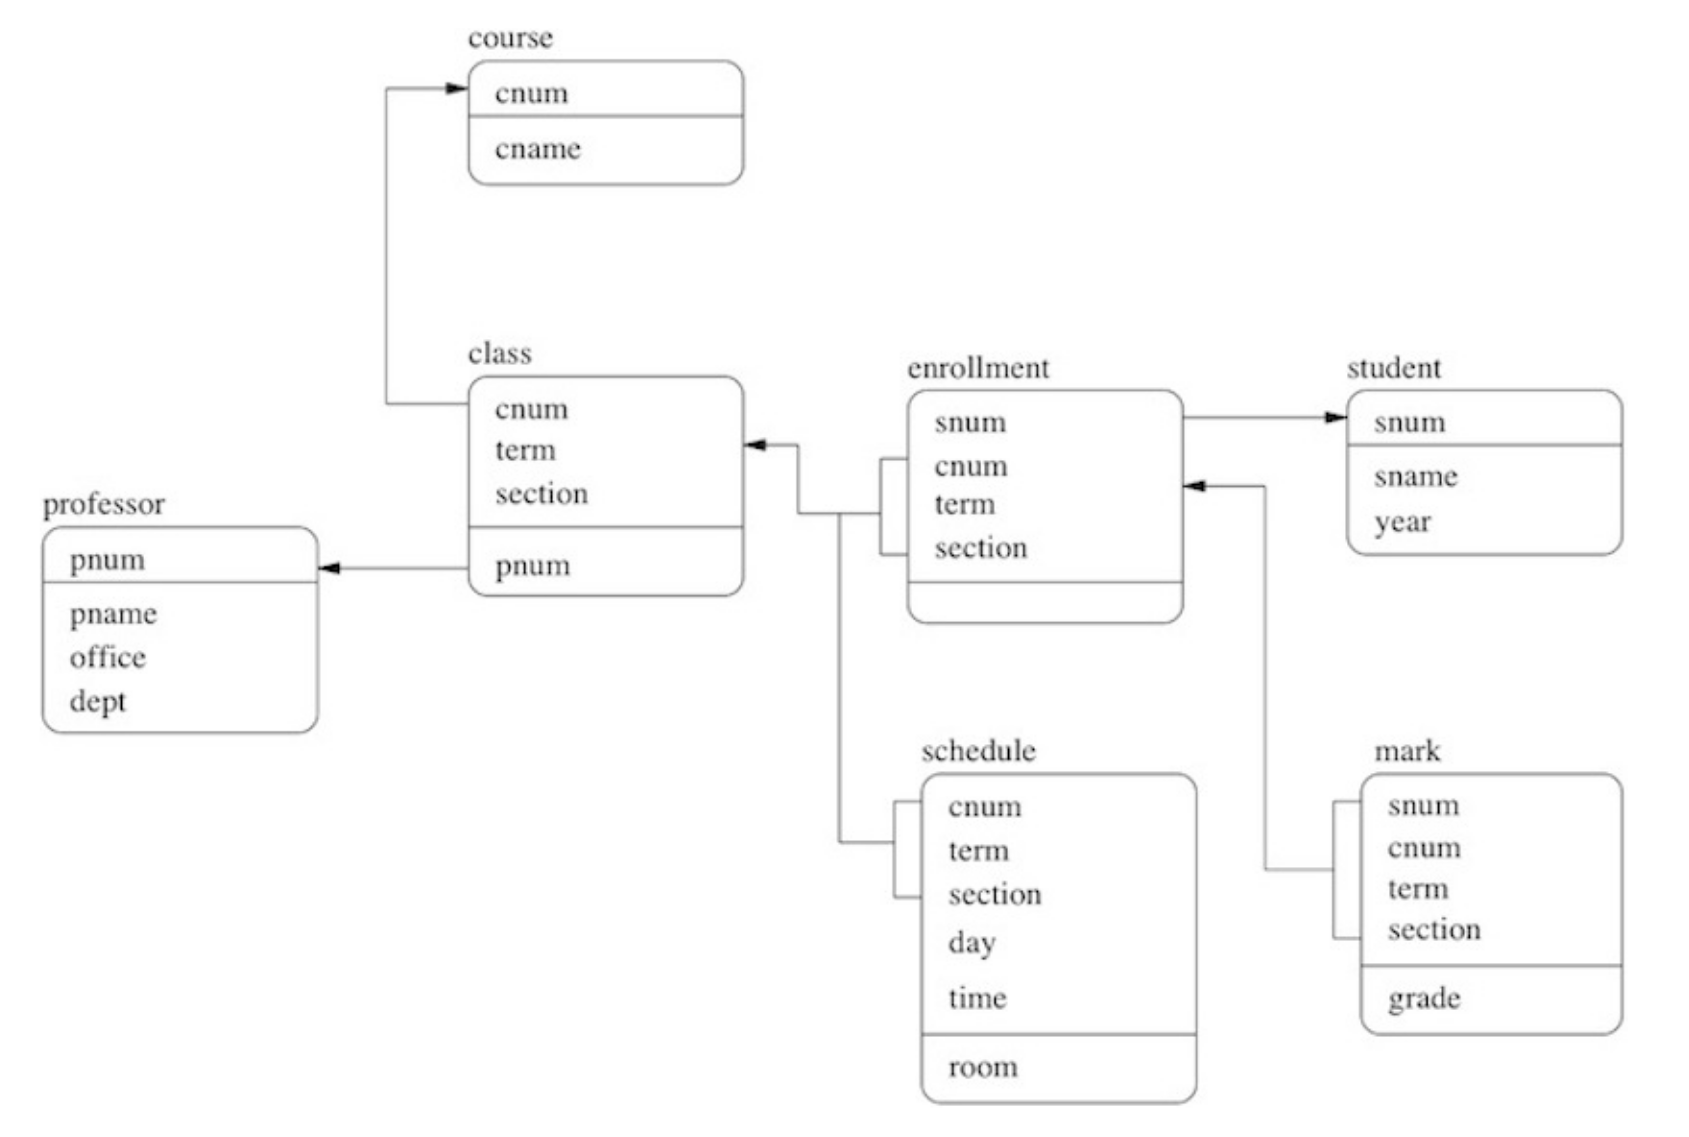
\includegraphics[width=0.9\textwidth]{images/db-schema.png}
\end{center}

\end{frame}


\begin{frame}
\frametitle{Let's get some exercise! - Relational Queries}

Find the names of all of the students that have not yet been given a grade in a class they have enrolled in.

Try writing the query in SQL, then in relational algebra.

\begin{center}
  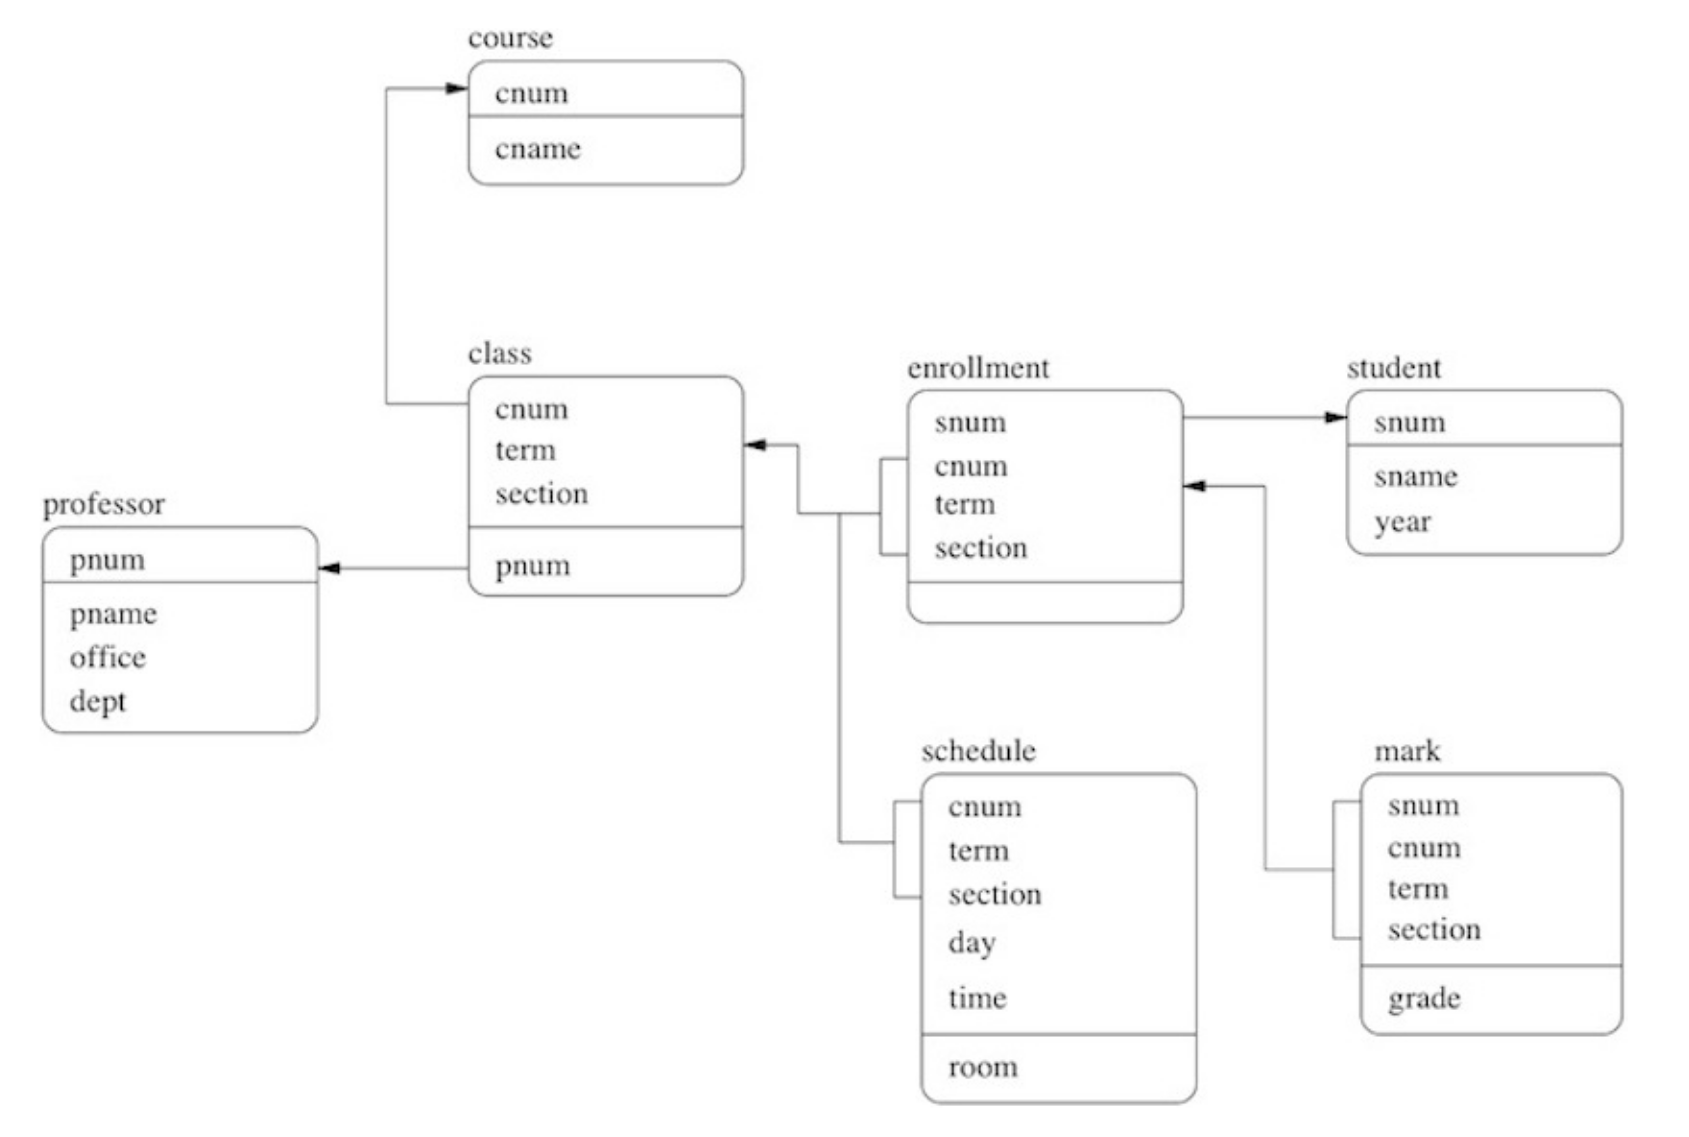
\includegraphics[width=0.9\textwidth]{images/db-schema.png}
\end{center}

\end{frame}


\begin{frame}
\frametitle{Let's get some exercise! - Relational Queries}

Find all of the course codes along with the names of a student with the top grades in each course.

Try writing the query in SQL, then in relational algebra.

\begin{center}
  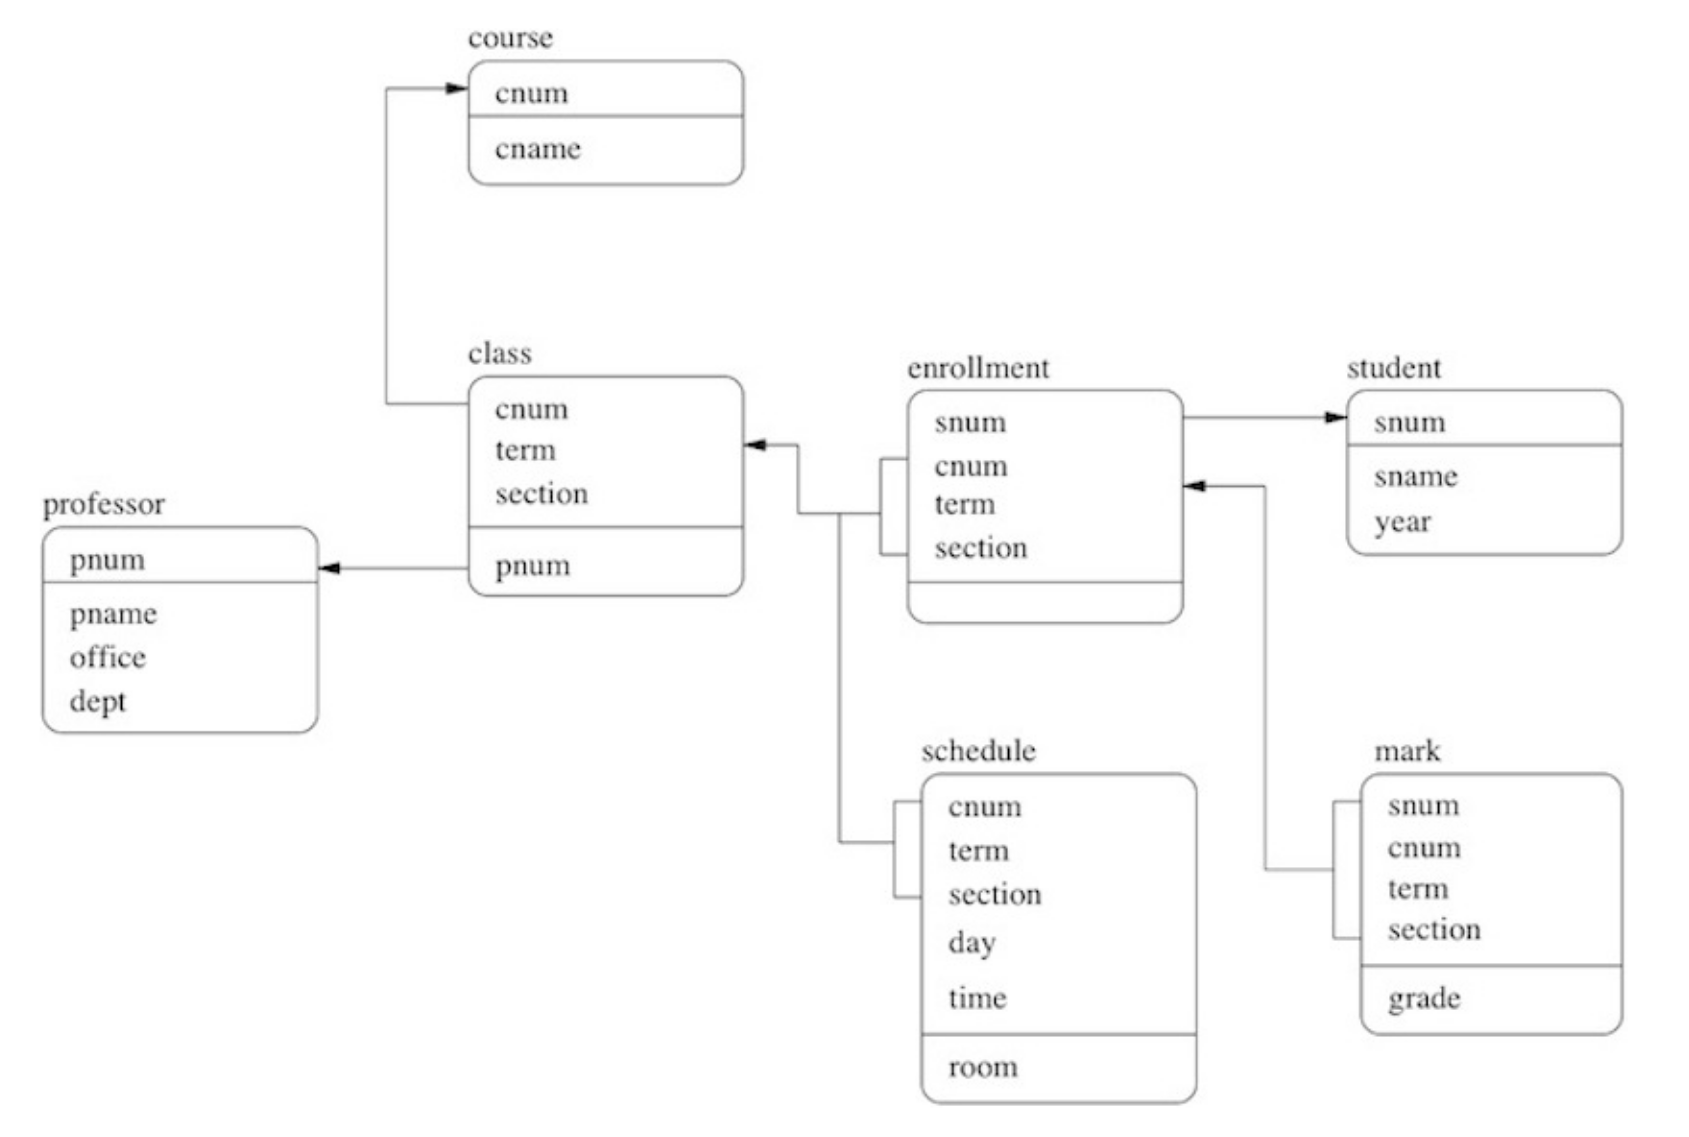
\includegraphics[width=0.9\textwidth]{images/db-schema.png}
\end{center}

\end{frame}
\end{document}
